\section{Side by side comparison between analysis results}
\label{sec:sidebyside}

\begin{figure}[H]
\hspace{-10mm}
  \subfigure[Theoretical analysis]{% 
    \includegraphics[width=.66\textwidth]{mat/antes_mat.png}
  } 
  \subfigure[Simulation analysis]{% 
    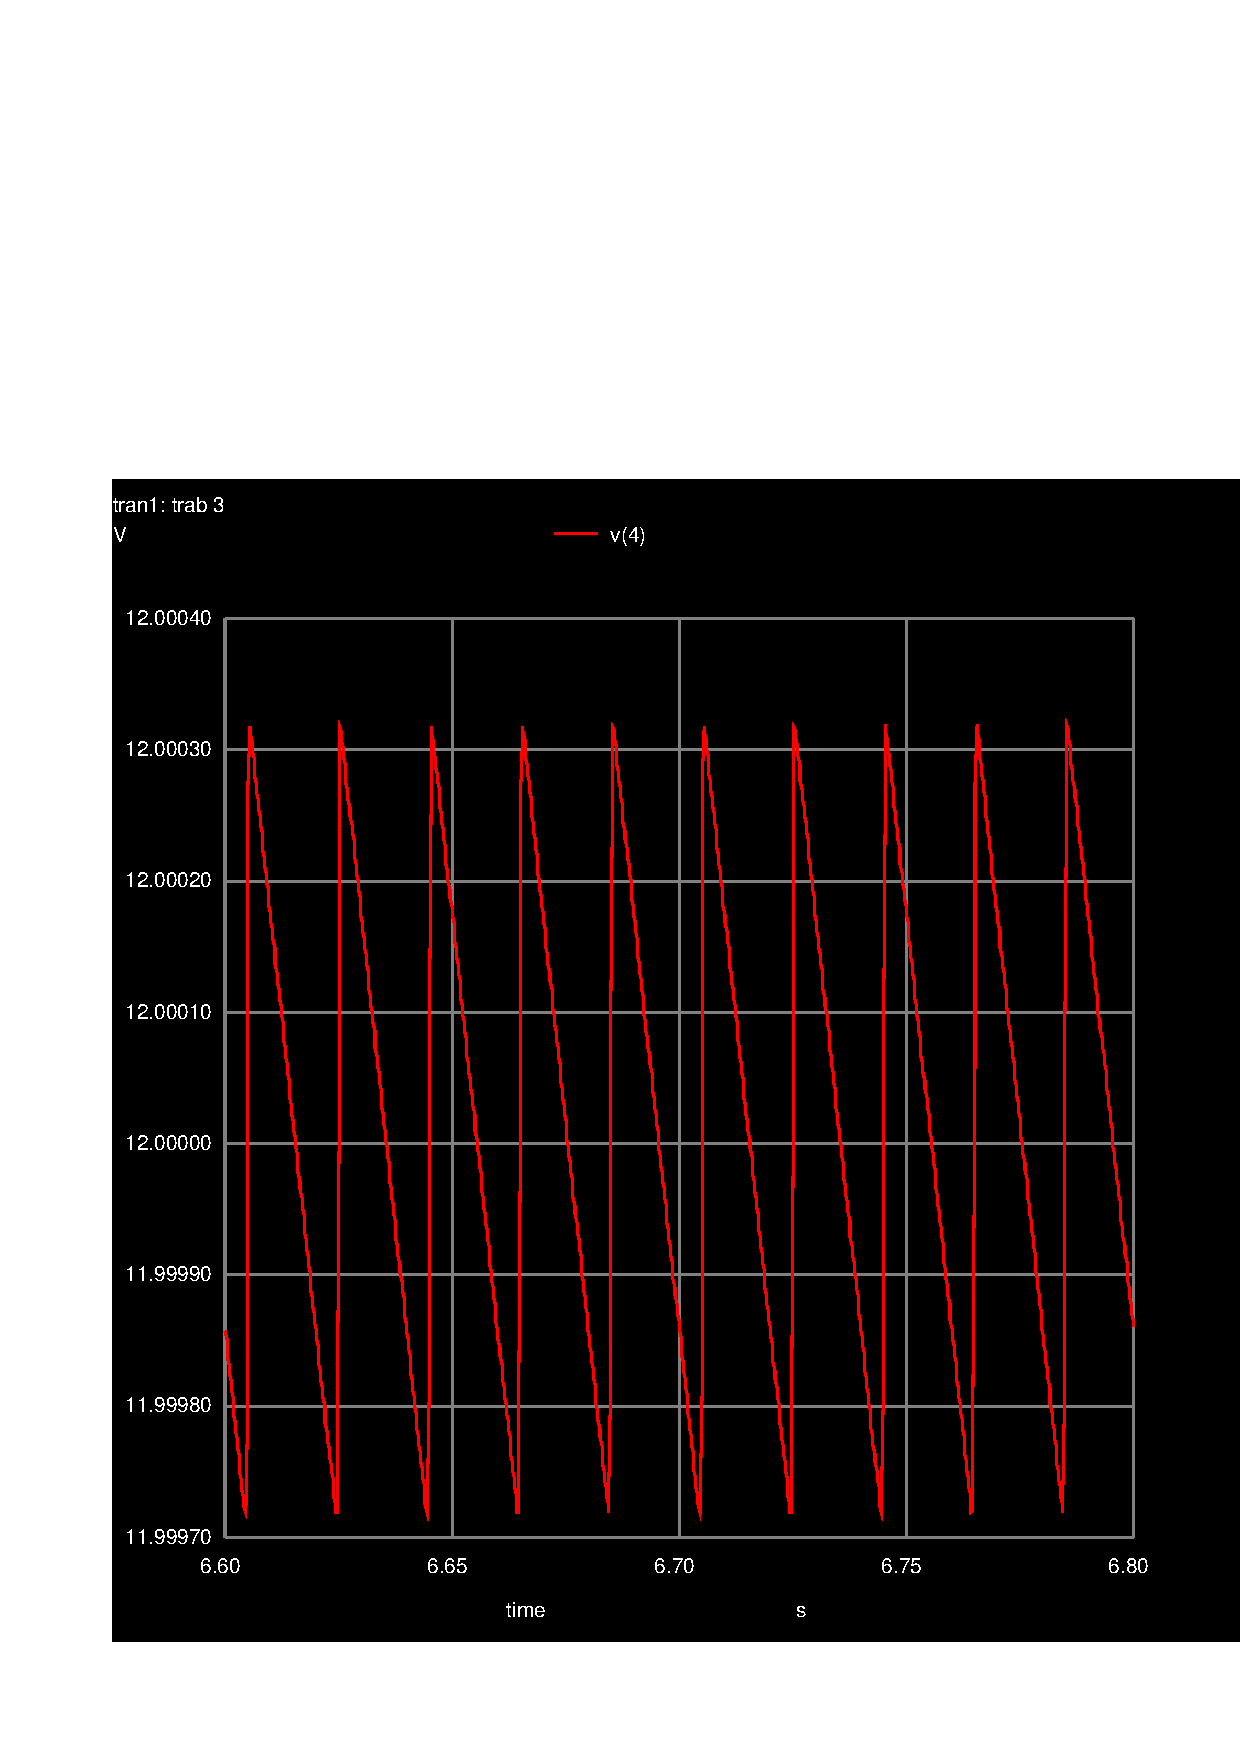
\includegraphics[width=.45\textwidth]{sim/antes.pdf}
  } 
  \caption{Signal as it exits the envelope detector.} 
\end{figure}

We can see that the signal has a similar shape although in the simulation analysis it is considerably bigger, once the circuit was optimized for the simulation analysis.

\begin{figure}[H]
\hspace{-10mm}
  \subfigure[Theoretical analysis]{% 
    \includegraphics[width=.66\textwidth]{mat/zauzau_mat.png}
  } 
  \subfigure[Simulation analysis]{% 
    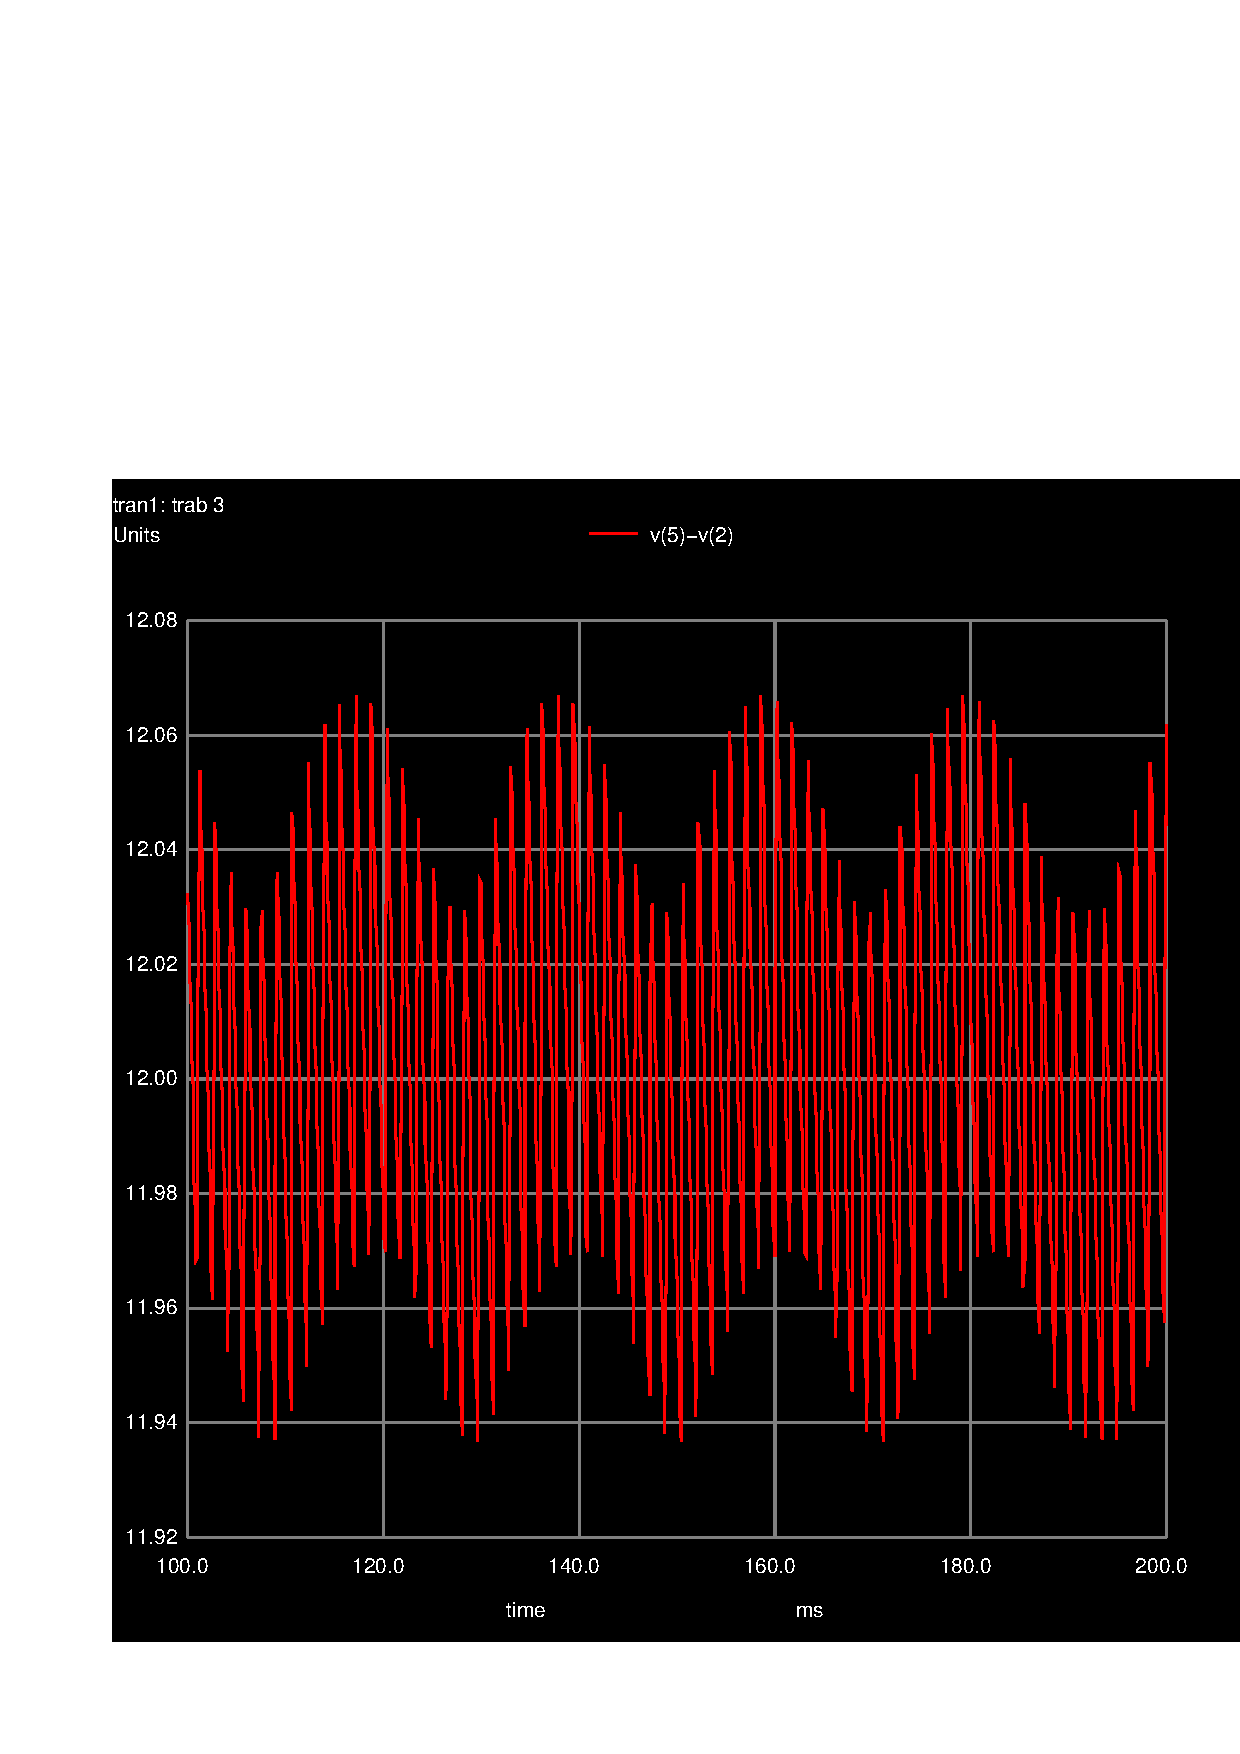
\includegraphics[width=.45\textwidth]{sim/zauzau.pdf}
  } 
  \caption{Output signal.} 
\end{figure}

The signal changes very little between the signal before and after the diodes and this difference is even smaller in the theoretical analysis because the resistance in the diodes is very high.

\begin{figure}[H]
\hspace{-10mm}
  \subfigure[Theoretical analysis]{% 
    \includegraphics[width=.66\textwidth]{mat/deviation_mat.png}
  } 
  \subfigure[Simulation analysis]{% 
    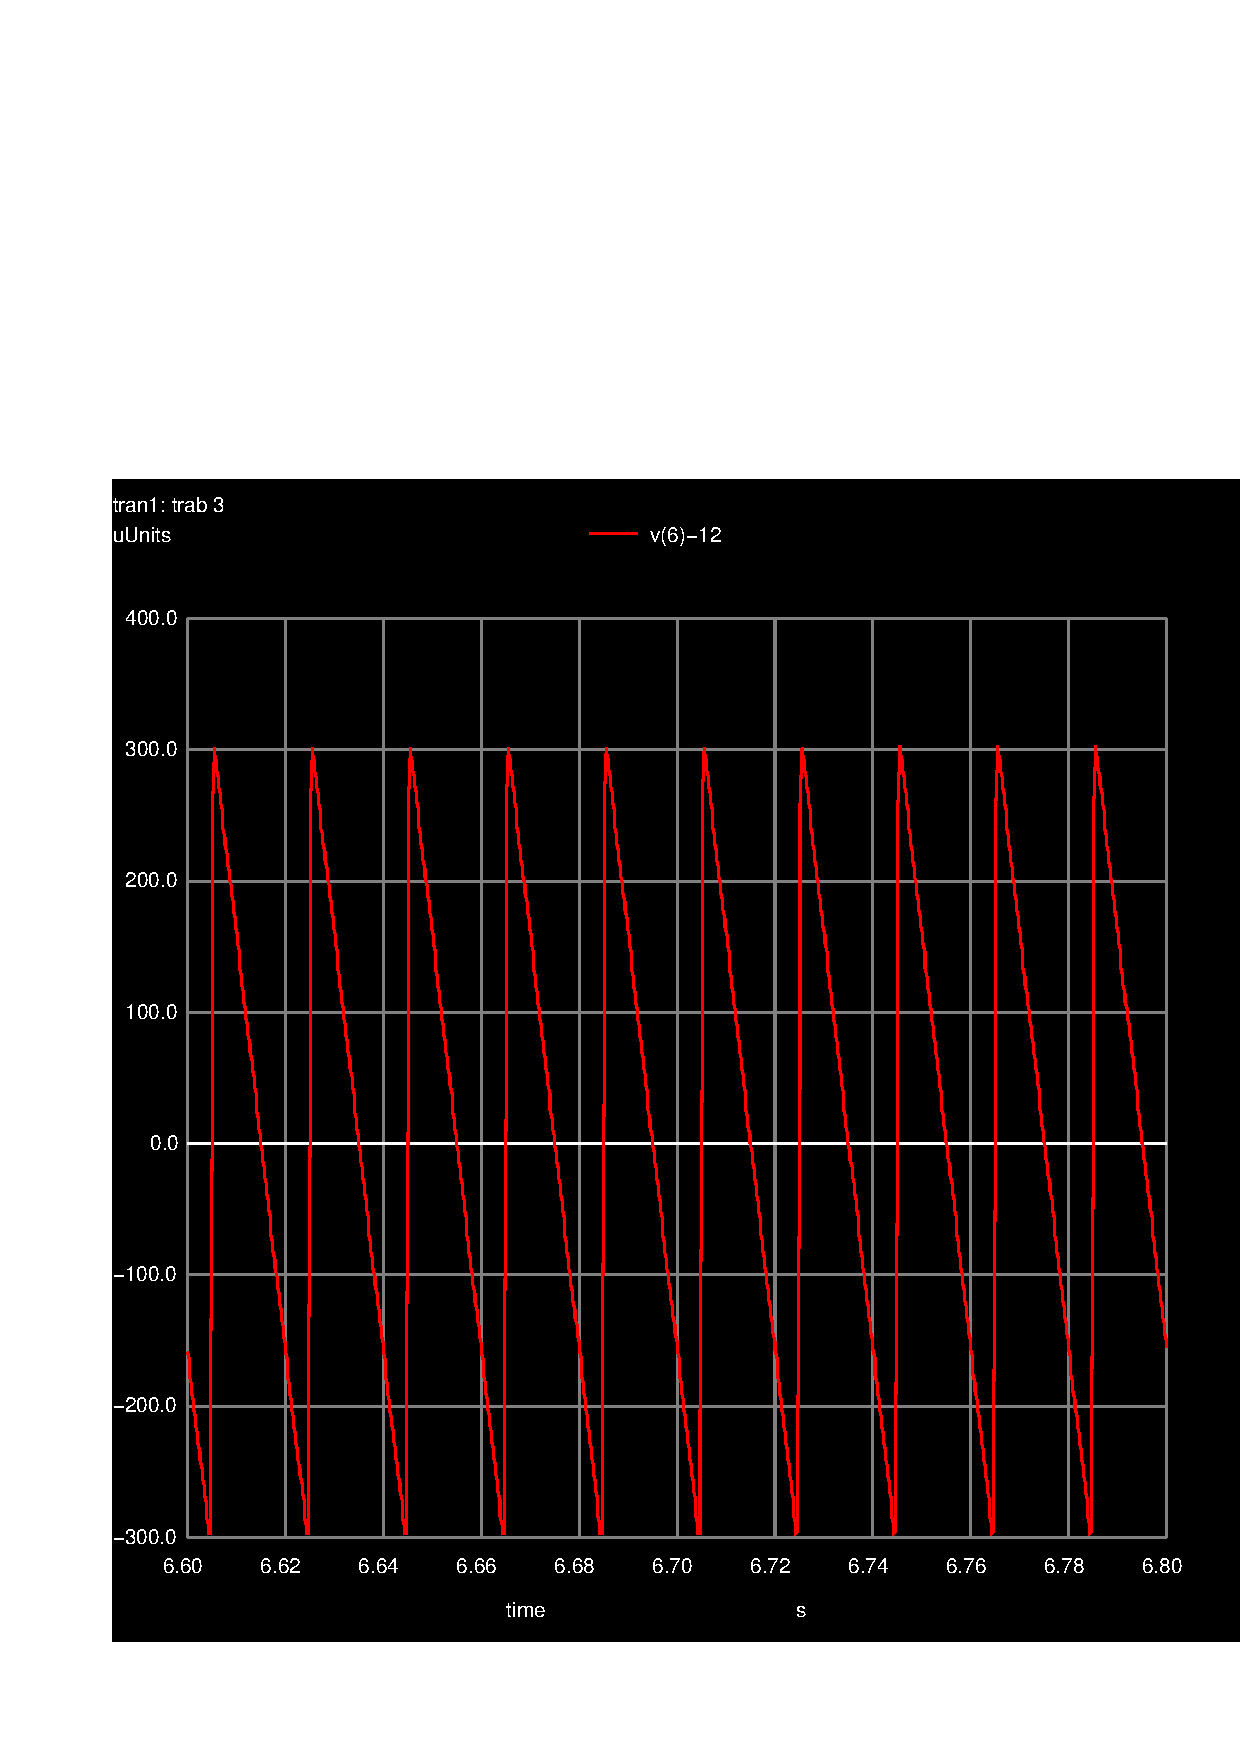
\includegraphics[width=.45\textwidth]{sim/deviation.pdf}
  } 
  \caption{Output signal minus 12, which should give only the deviations from the goal.} 
\end{figure}

The same comments as before can be made, but average voltage is not the one we want, being closer to 13 than 12.

\begin{figure}[H]
\hspace{-10mm}
  \subfigure[Theoretical analysis]{% 
    \includegraphics[width=.66\textwidth]{mat/acdc.png}
  } 
  \subfigure[Simulation analysis]{% 
    \includegraphics[width=.45\textwidth]{sim/acdc.pdf}
  } 
  \caption{Comparison between input and output voltage.} 
\end{figure}

On the big scale we can once again say that the the results are similar with the exception of the offset in the theoretical analysis.

\begin{table}[H]
    \begin{minipage}{.5\textwidth}
    \centering
    \begin{tabular}{|c|c|}
          \hline
          Average & \input{media}\\
          \hline
          Ripple & \input{ripple}\\
          \hline
          Merit &  \input{merit}\\
          \hline
          Corrected Merit & 1106.692837\\
          \hline
    \end{tabular}
    \caption{Theoretical analysis.}
    \end{minipage}
    \begin{minipage}{.5\textwidth}
        \begin{table}[H]
        \centering
        \begin{tabular}{|c|c|}
              \hline
              @gb[i] & -2.82647e-04\\ \hline
@id[current] & 1.016742e-03\\ \hline
@r1[i] & -2.69487e-04\\ \hline
@r2[i] & -2.82647e-04\\ \hline
@r3[i] & -1.31599e-05\\ \hline
@r4[i] & -1.17175e-03\\ \hline
@r5[i] & -1.29939e-03\\ \hline
@r6[i] & 9.022631e-04\\ \hline
@r7[i] & 9.022631e-04\\ \hline
v(1) & 7.795262e+00\\ \hline
v(2) & 7.515011e+00\\ \hline
v(3) & 6.927322e+00\\ \hline
v(4) & 2.756787e+00\\ \hline
v(5) & 7.555303e+00\\ \hline
v(6) & 1.145524e+01\\ \hline
v(7) & 9.222643e-01\\ \hline
cfp1 & 9.222643e-01\\ \hline

              \hline
        \end{tabular}
        \caption{Simulation analysis}
        \label{tab:fresnel2}
    \end{table}
    \end{minipage}
    \caption{Relevant values for our goal.} 
\end{table}

The corrected merit is just for adjusting the offset in the theoretical analysis. The real merit is of course way better in the simulation  analysis, because the circuit was developed in order to obtain the biggest merit possible but specifically for \textit{Ngspice}.